\chapter{Конструкторский раздел}
\label{cha:design}

В данном разделе будут приведены схемы конвейерной и линейной реализаций алгоритмов обработки матриц, приведено описание используемых типов данных, а также описана структура ПО.

\section{Схемы алгоритмов}

На рис. \ref{fig:linear_processing} - \ref{fig:stages} приведены схемы линейной и конвейерной реализаций алгоритмов обработки матрицы, схема трёх лент для конвейерной обработки матрицы, а также схемы реализаций этапов обработки матроицы.


\begin{figure}[h]
	\centering
	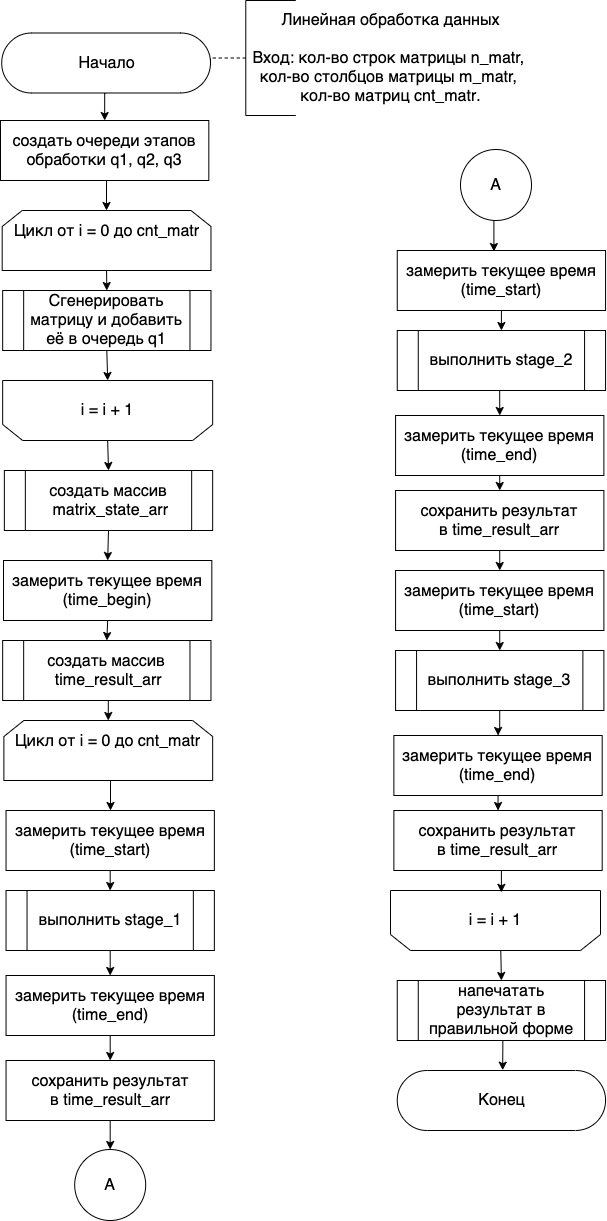
\includegraphics[scale=0.55]{img/linear_processing.png}
	\caption{Схема алгоритма линейной обработки матроицы}
	\label{fig:linear_processing}
\end{figure}

\clearpage

\begin{figure}[h]
	\centering
	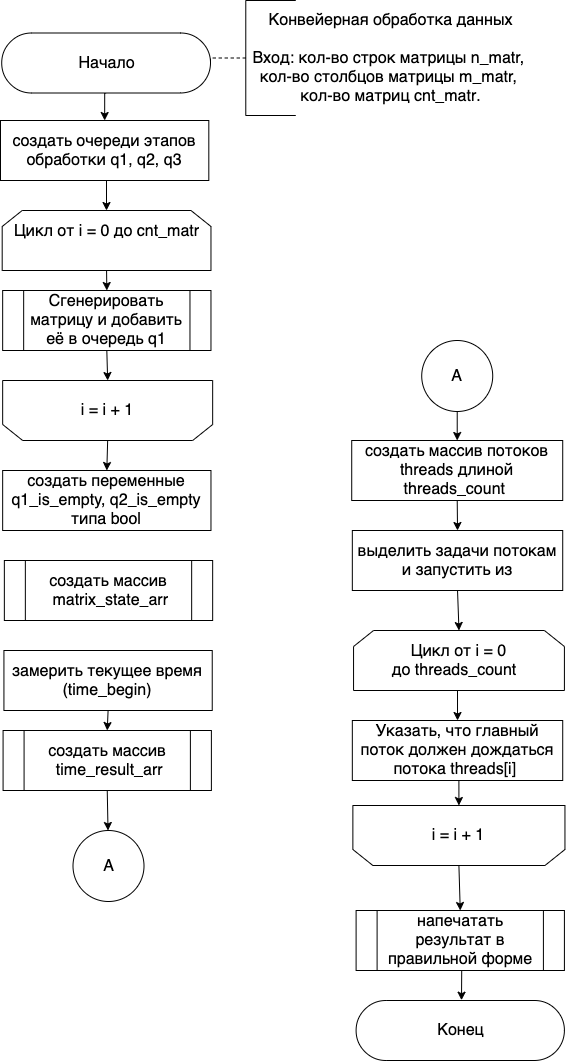
\includegraphics[scale=0.6]{img/parallel_processing.png}
	\caption{Схема алгоритма конвейерной обработки матроицы}
	\label{fig:parallel_processing}
\end{figure}

\clearpage

\begin{figure}[h]
	\centering
	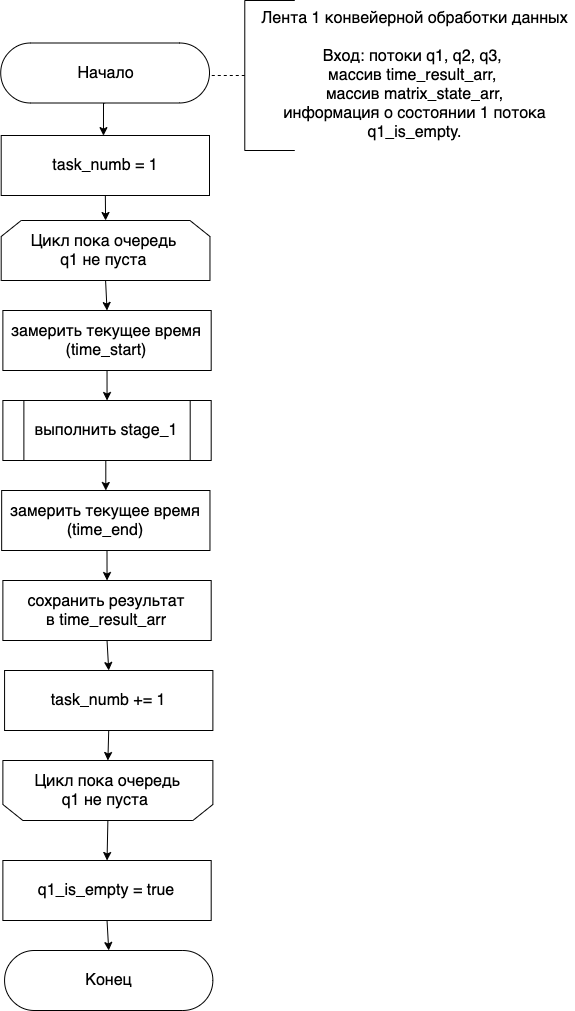
\includegraphics[scale=0.6]{img/parallel_stage_1.png}
	\caption{Схема 1-ой ленты конвейерной обработки матрицы}
	\label{fig:parallel_stage_1}
\end{figure} 

\clearpage

\begin{figure}[h]
	\centering
	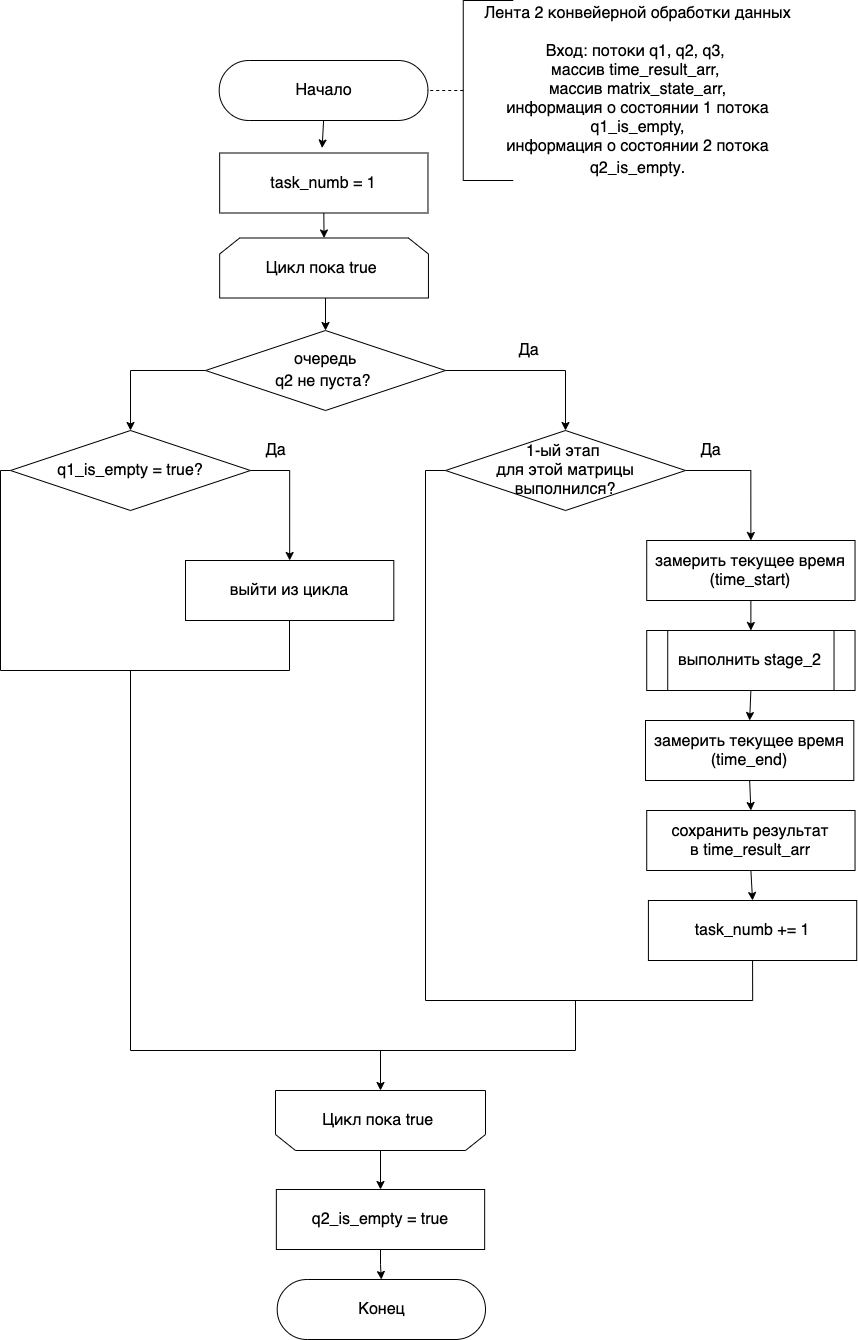
\includegraphics[scale=0.5]{img/parallel_stage_2.png}
	\caption{Схема 2-ой ленты конвейерной обработки матрицы}
	\label{fig:parallel_stage_2}
\end{figure} 

\clearpage

\begin{figure}[h]
	\centering
	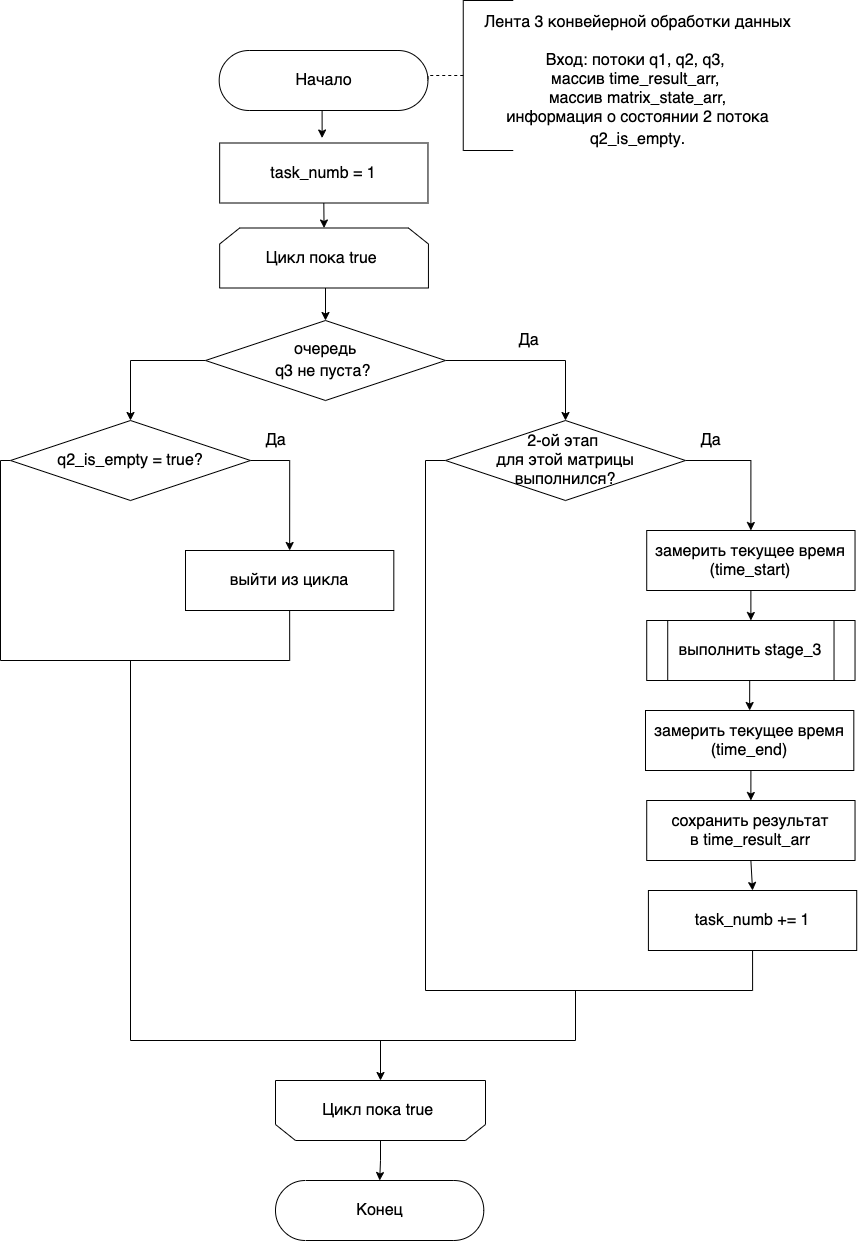
\includegraphics[scale=0.5]{img/parallel_stage_3.png}
	\caption{Схема 3-ей ленты конвейерной обработки матрицы}
	\label{fig:parallel_stage_3}
\end{figure} 

\clearpage

\begin{figure}[h]
	\centering
	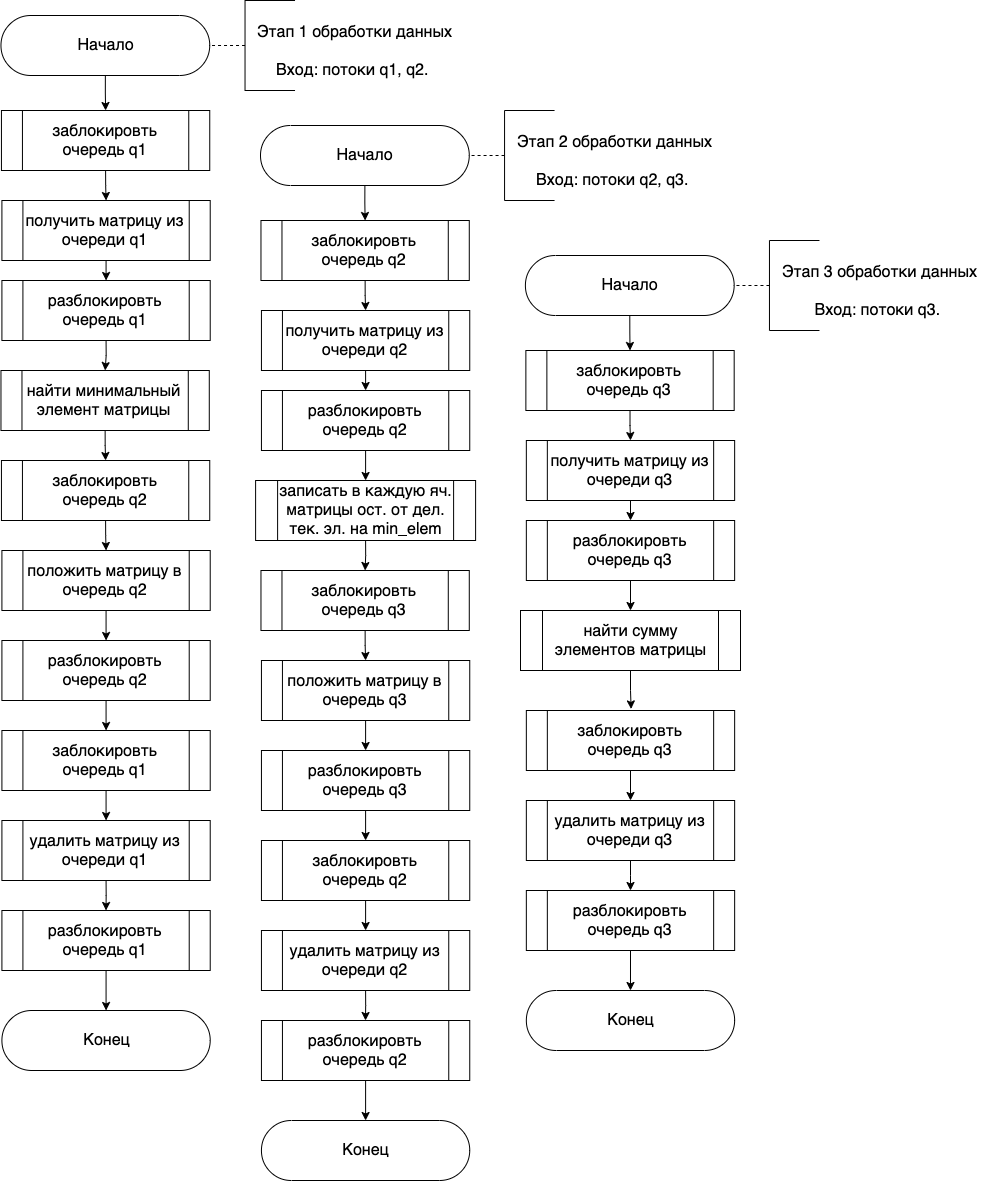
\includegraphics[scale=0.5]{img/stages.png}
	\caption{Схема реализаций этапов обработки матроицы}
	\label{fig:stages}
\end{figure} 

\clearpage

\section{Классы эквивалентности}

Выделенные классы эквивалентности для тестирования:

\begin{itemize}
	\item количество строк матрицы <= 0;
	\item количество столбцов матрицы <= 0;
	\item количество строк матрицы не является целым числом;
	\item количество столбцов матрицы не является целым числом;
	\item количество обрабатываемых матриц <= 0;
	\item количество обрабатываемых матриц не является целым числом;
	\item номер команды < 0 или > 3;
	\item номер команды не является целым числом;
	\item корректный ввод всех параметров;
\end{itemize}

\clearpage

\section{Структура ПО}

ПО будет состоять из следующих модулей:

\begin{itemize}
	\item main.cpp -- файл, содержащий функцию main;
    \item matrix.cpp -- файл, содержащий функции для работы с матрицей;
    \item compare.cpp -- файл, в котором содержатся функции для замера времени работы алгоритмов;
    \item read.cpp -- файл, в котором содержатся функции ввода данных;
    \item conveyor.cpp -- файл, в котором содержатся функции для конвейерной и линейной обработок матриц;
\end{itemize}

\section{Вывод}

В данном разделе на основе теоретических данных были построены схемы требуемых методов обработки матриц (конвейерного и линейного), выбраны используемые типы данных, выделены классы эквивалентности для тестирования, а также была описана структура ПО.

%%% Local Variables:
%%% mode: latex
%%% TeX-master: "rpz"
%%% End:
